\glsresetall

\chapter{Introduction}
\label{cha:intro}


Over the last three decades, technological advances have changed the way people use public transport. Before \gls{rti}, travellers would time their arrival at bus stops based exclusively on the bus's scheduled arrival time. There was no way of knowing if the bus was on-time, running late, or indeed if it was on its way at all until it finally appeared around the corner. These days, however, travellers can check the location of a bus from their phones before leaving home. Despite the accessibility of such \gls{rti}, unforeseeable traffic situations and various bus behaviours make estimating arrival times from vehicle locations a challenging task.


Around the world, public transport providers have invested in systems to provide \gls{rti} to travellers. Research has found that travellers perceive shorter wait times compared to their actual wait times in the presence of an arrival time countdown \citep{TCRP_2003}. \citet{Cats_2015} and \citet{Lu_2017} further reported that passengers who use \gls{rti} have shorter actual wait times on average than those who do not. However, as we shall see, \glspl{eta} may be unreliable, which is likely to frustrate passengers rather than appease them. For this reason, improving the \emph{reliability} of \gls{rti} is crucial for increasing \emph{ridership}, the number of passengers using public transport.


One limitation of \gls{rti} is the infrastructure required to keep track of vehicles and relay information to commuters \citep{TCRP_2003b}. As fleet sizes increase (over 1000~vehicles in Auckland), so to do the demands of \glspl{atis}, which has led some providers, notably Auckland Transport, to use the simplest of arrival time prediction frameworks. This simplification consequently results in less reliable systems, as I will discuss in \cref{sec:auckland_etas}.


The history of \gls{rti} for public transport spans several decades, which we will now examine, focussing on the key concepts essential for reliable \glspl{eta}. Afterwards, the current state of arrival time prediction in Auckland, New Zealand, is examined to establish why---despite decades of research---there is room for significant improvement. Finally, I present the aims of this research and summarize the process of estimating the arrival time of buses.



\section{A brief history of real-time information}
\label{sec:literature}

For a long time, public transport services such as buses and trains had only static timetables that passengers would use to plan their journey. There was no way for passengers to know if their bus was on-time, late, or early, nor could operators track how their services were running. In the 1960s, the first vehicle tracking systems were trialled in Germany and the United States of America \citep{TCRP_1997}. These early systems used \emph{beacons} (on signposts) placed along the route that the bus could detect, allowing it to provide its location to the service provider in real-time. Similar vehicle tracking technologies continued to develop over the subsequent decades; however, the focus remained on service monitoring and operational control.


The earliest uses of \gls{avl} technology for passenger information were \glspl{dms} at bus stops displaying a countdown to the next bus's arrival \citep{TCRP_2003}. One early example of this was Transport for London's \emph{Countdown} system \citep{Balogh_1993} which used the beacon (or signpost) \gls{avl} technology to determine vehicle locations and predict arrival times at bus stops.


Other vehicle tracking methods have since emerged using a range of technologies, the most notable being the widely used \gls{gps} \citep{Zhao_1997}. One significant advantage of the \gls{gps} is that it does not require fixed infrastructure (as does the signpost technology), making it easy for transit providers to add new routes or reroute existing ones without breaking the \gls{avl} system. A disadvantage of the \gls{gps} is that, rather than receiving \emph{route-specific} positions (``Signpost 8'', for example) the observations are \emph{map coordinates} which require an additional step to match them to the route.\footnote{Route matching and the issues associated with it are discussed in depth in later chapters.}


\citet{Cathey_2003} proposed a general prescription for making real-time arrival time estimates from \gls{gps} vehicle location data consisting of three components. First, a \emph{tracker} matches observations to scheduled \emph{trips} (time-specific instances of a route), which involves mapping \gls{gps} observations to the \emph{route path} to calculate the bus's \emph{trip-distance-travelled} (the distance the bus has driven along the route). Second, a \emph{filter} estimates the underlying vehicle state (which includes speed) that can be updated in real-time as new observations are received. \Citeauthor{Cathey_2003} used a Kalman filter for this step due to its superior real-time performance and previous use modelling the state of transit vehicles \citep{Wall_1999, Dailey_2001}. In the final \emph{prediction} component of their prescription, \citeauthor{Cathey_2003} used the estimated vehicle state in conjunction with travel time forecasts (estimated from historical data) to predict \emph{time until arrival}.


Some \gls{avl} systems report the vehicle's arrival and departure times from \emph{time points} (which are usually a subset of specific stops), providing observations of travel time between them. This type of reporting led to a range of new methods of arrival time prediction. For example, \gls{ann} and \gls{svm} models were implemented to predict travel time \citep{Jeong_2005,Shalaby_2004,Yu_2011,Cats_2015,Cats_2016,Yin_2017}. Many of these were in-depth research projects with access to high-quality data, such as high-frequency polling (10~seconds or less) or video footage, providing high-accuracy estimates of arrival and departure times. Despite their differences, all the approaches emphasize the importance of two components to arrival time prediction: \emph{travel time} between stops (or time points), and \emph{dwell time} (time spent at a stop while passengers board and disembark).


The concept of travel time between time points forms the foundation of arrival time prediction, so the estimation or forecasting of travel times has been the focus of much research. Returning to Transport for London's \emph{Countdown} system, \citet{Reinhoudt_1997} stored real-time travel times between time points in a database. They then used a \kf{} to update link travel times, significantly improving the accuracy of arrival time prediction. Others used historical data to estimate \emph{time until arrival} given a vehicle's trip-distance-travelled and speed \citep{Wall_1999,Dailey_2001,Cathey_2003}. Further improvements to prediction accuracy were obtained when real-time travel times along links were updated using a \kf{}, as it was capable of reacting to changes to traffic conditions \citep{Shalaby_2004}.


\Gls{ann} and \gls{svm} models have also been used to predict arrival time. \Citet{Yu_2006} demonstrated the feasibility and applicability of an \gls{svm} to predict travel time based on the bus's travel time along the current segment and the travel time of the most recent bus along the next segment. The limitation was that the model was trained for only one single route and only provided an arrival time for the next time point. \citet{Yu_2010} proposed an improved hybrid model using an \gls{svm} to model baseline travel time and a \kf{} to incorporate real-time data. Once more, this was limited to a single route and single-interval but demonstrated the importance of using real-time data for arrival time prediction. The next significant result was from \citet{Yu_2011} when they demonstrated the use of data across multiple routes to predict arrival time. In their study, \citeauthor{Yu_2011} used the travel times of recent buses between an automatic toll reader and a specific bus stop. While not generalised, they demonstrated the advantage of combining data across routes.


\Citet{Yin_2017} presented a model to predict travel time between stops using the travel times of previous buses from multiple routes, in which they chose two overlapping routes and manually identified common stops. They were able to predict travel time reasonably well, though both their \gls{svm} and \gls{ann} models failed to capture the peak period congestion. An alternative to machine learning models was proposed by \citet{Chen_2014}, who used a \emph{particle filter}\footnote{While their particle filter is unrelated to ours, the general methodology is the same and described in \cref{sec:recursive-bayes}.} to predict car travel time along roads from a database of historical data. Another unique approach by \citet{Julio_2016} used the concept of \emph{traffic shock waves} to predict travel times of buses along links based on the travel time along adjacent links. They used \gls{gps} observations to calculate vehicle trajectories over time and developed an \gls{ann} to learn patterns. As congestion builds along a segment, so too does congestion along the segment before it, for example.


Most of the methods described above only provide predictions for travel time along the next link, so arrival times are not available for stops further down the route. \Citet{Chang_2010} developed a \gls{knn} algorithm trained on historical vehicle trajectories to predict travel time along multiple upcoming links for a single route at a speed of 4000~predictions per minute.


Since the travel time of previous buses had been shown to improve arrival time predictions, other sources of information were explored to improve prediction accuracy further. This additional information could be significant along roads with low-frequency trips or subject to fast-changing traffic conditions. \Citet{Xinghao_2013} and \citet{Ma_2019} incorporated real-time taxi data to model traffic state. While this showed improvements, it is limited to locations with open access to taxi data.


Another source of uncertainty in arrival time comes from \emph{dwell time}, the time taken for passengers to board and disembark, at stops. \Citet{Shalaby_2004} showed that dwell times could have a substantial influence on arrival times. Along with a \kf{} for link travel times (each link consisted of 2--8~stops), \citeauthor{Shalaby_2004} also implemented a \kf{} on stop dwell times, allowing them to respond to real-time demand fluctuations which they measured using \glspl{apc}. Other work has also demonstrated the necessity of incorporating dwell times into arrival time predictions \citep{Jeong_2005,Cats_2015,Cats_2016}.


When it comes to modelling transit vehicles and predicting arrival times, there is a lot of uncertainty in vehicle trajectories, particularly when observations are sparse. Additionally, much of this uncertainty is non-Gaussian (particularly multi-modal). \Citet{Hans_2015} presented a particle filter for modelling transit vehicles that incorporates bus stop dwell times and traffic light phasing using data from \gls{gps} devices and \glspl{apc}. The primary advantage of the particle filter over other methods (such as the \kf{}) is its ability to sample a wide range of plausible trajectories, which is of particular importance as uncertainty increases for later stops. The distribution can also be strongly multi-modal due to buses not necessarily stopping at all stops.\footnote{I will demonstrate this in more detail in the coming chapters.}


Since uncertainty is an unavoidable component of arrival time prediction, some attempts at conveying this to travellers have been explored. \Citet{Mazloumi_2011} assessed the use of \emph{prediction intervals} obtained from an \gls{ann} model, focussing on the accuracy (coverage) of these intervals. A unique approach was demonstrated by \citet{Fernandes_2018} that involved displaying \emph{uncertainty graphs}---including quantile dot plots---and found that their test subjects made better decisions when they had uncertainty information.


The final component of \gls{rti} that we are interested in is \emph{journey planning}, which involves the selection of an optimal route to get to a destination, often under one or more constraints. \Citet{Horn_2004} developed a real-time routing method that could incorporate \emph{walking} and \emph{waiting costs} (each of these should be minimised where possible), with a focus on \emph{demand-responsive} services. More recently, \citet{Hame_2013a,Hame_2013b} proposed a \emph{Markov decision process} which could maximise the probability of arriving at the destination on-time, accounting for walking legs and distributions for the arrival time of buses at stops.  \citet{Zheng_2016} incorporated travel time uncertainty into their method while also demonstrating the complexity of the problem:  it could take $10^3$~seconds to find an optimal route. Their solution was to store paths, reducing computations to less than a second. As an alternative to incorporating travel time uncertainty, \citet{Berczi_2017} present a dynamic routing strategy that uses any probabilistic model of arrival and departure times to improve the probability of arriving at the destination on time.


\section{The state of Auckland's RTI}
\label{sec:auckland_etas}

Our case study is the public transport system of Auckland, New Zealand, operated by Auckland Transport. In the following pages, I describe some scenarios that occur within Auckland,\footnote{Some of which I have personally witnessed.} although they likely occur in other cities that use the same \gls{avl} system (described in detail in \cref{sec:gtfs}). Additionally, many locations in Auckland lack transit infrastructure, such as bus priority lanes, which can lead to long delays during heavy congestion.


Other issues are related to driver behaviour and \emph{schedule adherence}. Auckland Transport itself does not actively monitor schedule adherence beyond the first stop: ``Punctuality is measured by the percentage of total scheduled services leaving their origin stop no more than one minute early or five minutes late'' \citep[13]{AT_report_2019}. As demonstrated in \cref{fig:schedule_adhere}, buses tend to run early, particularly towards the end of the route, which I would argue is more frustrating than running late for anyone wanting to catch it. At other times, travellers may need to catch multiple buses to get somewhere, in which case a \emph{transfer} between services is necessary. However, if the first bus runs late, the connecting bus will usually depart on time (before the first bus gets there) leaving the passenger stranded until the next trip. In some cases, this may be 30~minutes or more, which inevitably leads to frustrated passengers.\footnote{I have experienced this more than once, where the second bus for my trip home departed as the one I was on pulled into the station.}


\begin{knitrout}\small
\definecolor{shadecolor}{rgb}{0.969, 0.969, 0.969}\color{fgcolor}\begin{figure}
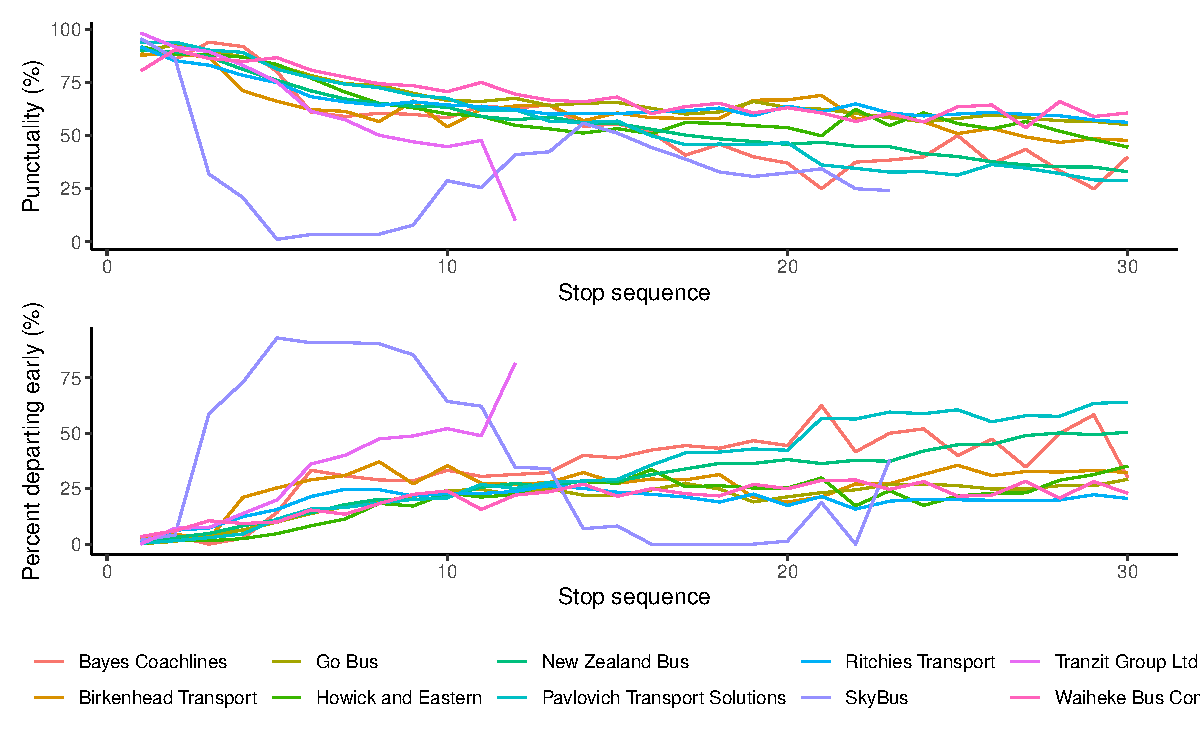
\includegraphics[width=\linewidth]{figure/schedule_adhere-1} \caption[Punctuality of Auckland's transport service providers]{Punctuality (top) and percentage of services arriving early (bottom) for Auckland's transport service providers by stop sequence. Punctuality is measured by the percentage of services departing between 1 minute early and 5 minutes late.}\label{fig:schedule_adhere}
\end{figure}


\end{knitrout}



Given that many of the issues with Auckland's transport system relate to infrastructure, the simplest solution is improved, reliable \gls{rti}. Auckland Transport uses \gls{gtfs}, a specification for how transit data should be organised \citep{GoogleDevelopers_2006}. Part of \gls{gtfs} provides a simple method for predicting arrival times, which is what Auckland Transport and other agencies use. In this method, \emph{trip updates} are reported when a bus arrives or departs from a stop, and includes the vehicle's \emph{delay} (the difference between scheduled and actual arrival). Arrival time at upcoming stops is then estimated by adding this delay to their scheduled arrival times. This method quickly runs into problems if the scheduled travel times are not accurate and drivers do not actively adhere to them.


Besides being inaccurate and unreliable, arrival times based on schedule and current delay are prone to sudden changes in the vehicle's delay. For example, if the bus encounters heavy traffic between stops, it will get later, but this is not reported to passengers until the bus finally arrives at the next stop. When it does, passengers waiting at stops farther along see the \gls{eta} suddenly increase. Another common occurrence is when the bus is delayed on a previous trip: the default arrival time estimate is the scheduled arrival time, so until the bus starts the trip, the \gls{eta} is as scheduled. When the bus is delayed, it may commence the route ten or more minutes late, and when it finally does, the \glspl{eta} at stops suddenly increase by ten (or more) minutes. If the \gls{eta} reaches zero before the bus begins the trip, the bus disappears from the \gls{dms} completely. These scenarios all contribute to traveller frustration and lack of trust in the system.


Conversely, \gls{gtfs} provides an opportunity for a standard, globally available framework: ``The standardised format means that innovative tools and products that utilize GTFS can easily be applied across transit agencies.'' \citep[26]{TCRP_2020}. It is therefore desirable to have a framework that is capable of using solely \gls{gtfs} data to model transit vehicles, estimate traffic conditions throughout the network, and predict arrival times. Location-specific features, such as taxis or intersection locations, should not be required, but could be added as necessary provided the framework is structured to allow it.


The components described in the literature as essential to arrival time prediction are travel time and dwell time. To the best of our knowledge, there is no system based solely on \gls{gtfs} data that provides a means of combining data across routes to estimate traffic conditions and use them to improve arrival time prediction.



\section{Research outline}
\label{sec:proposal}

Public transport is essential wherever people need to get to and from work, school, or other activities dependably. However, in this age of cellphones and \gls{rti}, travellers have come to expect, at the very least, a reliable countdown on the \gls{dms} at their stop. In Auckland, this is not the case. The unreliability of \glspl{eta} makes them unusable for real-time journey planning, causing difficulties for commuters who rely on public transport and potentially driving them to consider alternative---often private---transport options.


The central focus of this thesis is to develop an arrival time prediction application that accounts for real-time traffic information obtained from both static and real-time data provided by \gls{gtfs}. This means that the application can be applied to any city using \gls{gtfs}, and not solely Auckland, as many of the problems discussed will be present elsewhere. We explore how traffic state can be estimated independently of routes so that routes that use the same roads can share travel time or speed information. Our goal is to make arrival time predictions which, by accounting for real-time traffic conditions, are more reliable than those currently available in Auckland. However, it is clear from both the literature and personal experience that substantial levels of uncertainty are inescapable in transit prediction. For this reason, we focus on capturing the uncertainty in the model and estimating the \emph{arrival time distribution}, which can be summarized using, for example, prediction intervals.


We also consider journey planning, notably the use of arrival time distributions to make decisions, since Auckland (and other) transit providers offer no such service. Auckland Transport's ``journey planning'' is based solely on the scheduled timetables, as do transit directions provided by Google Maps\footnote{\url{https://maps.google.com}}. \Citet{Berczi_2017} demonstrate the use of probabilistic arrival time distributions in a real-time dynamic routing problem. It is not our intention to solve the routing problem (selecting candidate routes from origin to destination), but instead to demonstrate the reliability (or usefulness) of our arrival time distribution in choosing between alternative routes. This could then be incorporated into a dynamic routing framework that uses the probabilities of events to make decisions.


Before approaching this problem, I first provide an overview of the relevant background information in \cref{cha:data}. This includes an overview of \gls{gtfs} and a discussion of the characteristics of real-time transit data. We will also examine how a \emph{network} can be constructed from \gls{gtfs} data to allow the sharing of information across independent routes. Lastly, I give a brief introduction to \emph{recursive Bayesian filtering}, an approach to modelling data in real-time that is used extensively throughout this thesis.


Having laid some foundations, we begin the process of real-time prediction by first modelling the state of a transit vehicle, which is updated whenever new data is received. One important aspect of \cref{cha:vehicle_model} involves removing all unnecessary uncertainty. \Citet{Cathey_2003} (and others) used \emph{map-matching} to calculate the vehicle's trip-distance-travelled from the reported \gls{gps} coordinates. As part of the vehicle model, I propose a method of removing this step and incorporating \gls{gps} observations directly into the likelihood function to overcome several of the issues identified in \cref{cha:data}. The main goal of \cref{cha:vehicle_model} is to use real-time transit vehicle observations to estimate vehicle speed along roads. This is similar to the work of \citet{Celan_2017,Celan_2018} who used historical data to estimate average vehicle speed along roads in a \emph{network}.


After observing the speeds of transit vehicles travelling around Auckland, we can model the real-time \emph{traffic state} of the road network. Similar to the work of \citet{Shalaby_2004} we develop a \kf{} that allows real-time estimation of network state in \cref{cha:network_model}. A large part of this consists of estimating the necessary model parameters from historical data and assessing the real-time accuracy of our model. As many previous researchers have noted, predicting future travel times (which depend on road state) is difficult and requires a more complex model than the \kf{}. At the end of \cref{cha:network_model} I discuss a possible approach to forecasting that could later be incorporated into the arrival time prediction component of our application.


Finally, we come to arrival time estimation itself, which combines vehicle and road states to obtain an arrival time distribution. In \cref{cha:prediction}, I demonstrate how the distribution itself is computed and compare our approach to several others. Then, in \cref{cha:etas}, I derive a simplified arrival time \gls{cdf} and present several forms of summary statistics that could be displayed to commuters (point and interval estimates).  We also explore the use of the \gls{cdf} to answer journey planning questions concerning, for example, journey length or the probability of on-time arrival. These results focus on the reliability and potential usefulness of our method's predictions compared to those currently available in Auckland.


Since this is a real-time application, we assess its computational performance throughout. Therefore, at the end of each chapter, I describe the programmatic considerations of the application and discuss the relative components of the \Rstats{} package \pkg{transitr} developed as part of this research. The target for real-time predictions---from the time the data is first requested from the server until \glspl{eta} are available for travellers---is 30~seconds.


Finally, in \cref{cha:discussion}, we review our methods and findings and comment on what could be done to improve our application in the future. The role of \gls{rti} in public transport is only going to become more critical as cities---particularly Auckland---grow. Improving the reliability of the information is the first step to increasing ridership.
